\documentclass[paper=a4paper,fontsize=10pt,jafontscale=0.925,twocolumn]{jlreq}
\usepackage{luatexja}
\usepackage{lab-handout}
\usepackage{graphicx} % Added for includegraphics

% ここから上は変更しない

\title{VRコンテンツ体験時における生体・行動情報の統合に基づくリアルタイム感情推定フレームワーク} % 自身の卒業研究/修士論文の予定表題に変更

%以下は適切な所属を1つ選択
\affiliation{人間システム工学科 井村研究室} % 卒業研究(人間システム工学科)
%\affiliation{人間システム工学科 井村研究室} % 卒業研究(知能・機械工学課程)
%\affiliation{人間システム工学専攻 井村研究室} % 修士論文

\studentnumber{27020856} % 8桁の学籍番号
\author{趙 聖化} % 姓名間の空白は半角で

\graphicspath{{./}} % 画像を置いておくフォルダ名

\begin{document}

\maketitle

% ----- 図1(flowchart)のブロックを削除しました -----
% \begin{figure}[tp]
%  \centering
%  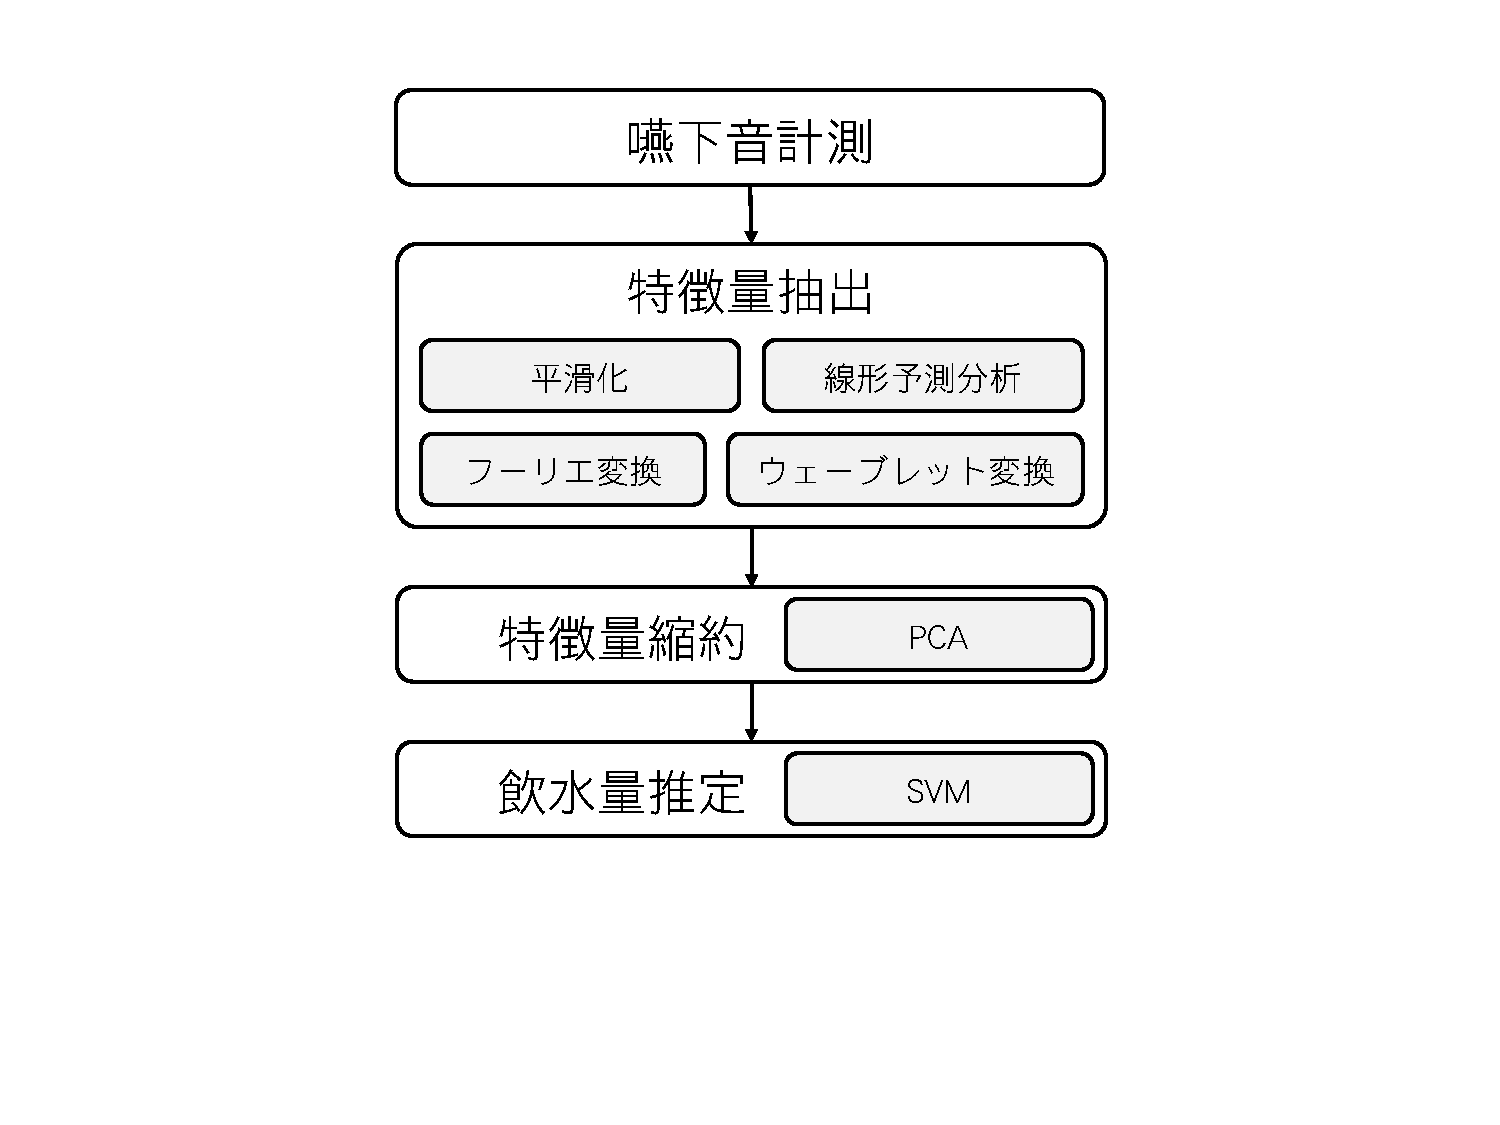
\includegraphics[width=\columnwidth]{flowchart.pdf}
%  \caption{提案する感情推定システムの処理フロー}
%  \label{fig:flow}
% \end{figure}

\section{はじめに}

VRコンテンツはさまざまに制作されていますが, その評価は主観的になりがちです.制作者の意図した感情が、実際にユーザーに伝わっているかどうかを客観的に把握することは難しいのが現状だ。視線追跡機能付きHMD(ヘッドマウントディスプレイ)と,皮膚電気活動(EDA)・心電(ECG)・筋電(EMG)などの複数の生体センサを統合し,VRホラーコンテンツを体験しているユーザの「集中」「恐怖」「驚き」といった感情状態を実時間で推定するフレームワークの構築をする 。

\section{関連研究}

生体信号を用いた感情推定は広く研究されている。EDAは情動的な覚醒度の指標として, 心拍変動(HRV)はストレスや感情の正負(valence)の評価に用いられている. 複数の生体信号を組み合わせることで,単一のセンサよりも高精度な感情推定が期待できる.

VR環境下で生体信号を計測し,機械学習を用いて感情を分類する試みも活発になされている。Marín-MoralesらはEEGとHRVからSVMを用いて覚醒度と感情価を推定した. また, Orozco-MoraらはVRゲーム中のストレスレベルに応じて難易度を動的に調整するシステム(DDA)を試作しており, プレイヤーの心拍数に基づいてゲーム内パラメータを変化させることで, 恐怖や興奮を適切なレベルに維持できることを示している.

\section{提案手法}

本研究では,HMDと複数の生体センサを連携させ,VRホラー体験中のユーザの感情を実時間で解析するシステムを構築する.

\subsection{システム構成とデータ収集}

視線・瞳孔径情報を取得可能なHMDを中核とし,外部センサとしてEDA(皮膚コンダクタンス),ECG(心拍),EMG(表情筋・筋緊張)センサを連携させる. 多角的データを用いて,「恐怖による心拍・発汗の上昇」「驚きによる瞬きや筋収縮」「集中による画面の凝視」といった各感情の兆候を捉える. 加えて,コントローラの加速度センサ情報や,驚愕反応としてのボタン入力(例:長押ししていたボタンを離す)も行動指標として取得する.客観データはVR内のイベントログと時刻同期させて記録し,体験後に実施するアンケートによる主観評価と合

\subsection{データ処理とリアルタイム推定}

収集した各センサデータから、リアルタイムで特徴量を抽出する。具体的には、EDAのピーク数、HRV指標(RMSSD:連続する心拍間隔差分の二乗平均平方根、LF/HF比:低周波/高周波成分比)、EMGの振幅、瞳孔径変化量、コントローラからの行動データなどである. 特徴量を入力とし,ランダムフォレストやSVM,LSTMなどの機械学習モデルを用いて,「安静」「警戒」「恐怖・驚愕」といった感情ラベルに分類する.

リアルタイム推定においては,各信号の時間的特性を考慮する. 例えば,心拍やEMGのような即時的な反応は1\textasciitilde2秒という短い時間窓で変化を捉え,EDAのような遅れて現れる反応は6\textasciitilde10秒という長めの時間窓でトレンドを見ることで,推定の安定性と応答速度の両立を図る.

\section{予備実験計画}

提案手法を検証するため,以下の予備実験を計画する 。

\begin{itemize}
    \item \textbf{目的:} 構築したシステムがVRホラーによる感情喚起を正しく捉えられるか確認し,特徴量と感情の関係性を予備的に検証する 。
    \item \textbf{被験者:} 5\textasciitilde10名程度の若年層ボランティアを対象とする.
    \item \textbf{手順:} VRホラーコンテンツを体験してもらい,その間の生体・行動データを記録する。体験後,アンケートにてシーンごとの主観的な恐怖度・驚き度・集中度を評価してもらう 。
    \item \textbf{分析:} 収集した生体・行動データと主観評価,およびイベントログとの相関を分析する.例えば,ジャンプスケア直後の心拍数やEDAの急上昇,コントローラの動きなどを確認する 。このデータを用いて,感情分類モデルの予備的な学習と評価を行う.
\end{itemize}

\section{まとめと今後の課題}

本稿では,VRコンテンツ体験時におけるユーザの感情を,複数の生体センサを用いて実時間で推定する研究フレームワークを提案した.

今後の課題として,まず提案システムの基盤構築と,予備実験の実施(2025年6\textasciitilde9月)を進める 。予備実験の結果に基づき,特徴量や機械学習モデルを洗練させた後,本実験と詳細な分析を行う(2025年10\textasciitilde11月) 。最終的には,本研究の成果を,ユーザの感情状態に応じてコンテンツが動的に変化する適応型VRシステムの実現に繋げることを目指す.

\begin{thebibliography}{9}

\bibitem{Guixeres2020}
J. Guixeres, et al., Emotion Recognition in Immersive Virtual Reality: From Statistics to Affective Computing, \textit{Frontiers in Psychology}, Vol. 11, 2020. 

\bibitem{Marin-Morales2018}
J. Marín-Morales, et al., Affective Computing in VR Environments using EEG and Heart Rate Variability, \textit{Sensors}, Vol. 18, No. 10, 2018. 

\bibitem{Orozco-Mora2024}
C.E. Orozco-Mora, et al., Dynamic Difficulty Adaptation Based on Stress Detection for a VR Video Game: A Pilot Study, \textit{Electronics}, Vol. 13, No. 12, 2024. 

\bibitem{Glancy2021}
M. Glancy and C.S. Ang, VREED: Virtual Reality Emotion Recognition Dataset using Eye Tracking \& Physiological Measures, \textit{Proc. ACM IMWUT}, Vol. 5, No. 4, 2021. 

\bibitem{Ogawa2014}
小川健一, 杉本泰治, 視線計測によるストレス評価手法の検討, \textit{日本バーチャルリアリティ学会論文誌}, Vol. 19, No. 1, pp. 61-70, 2014. 

\end{thebibliography}

\end{document}